%% Creator: Inkscape inkscape 0.48.4, www.inkscape.org
%% PDF/EPS/PS + LaTeX output extension by Johan Engelen, 2010
%% Accompanies image file 'numberofframessvg.pdf' (pdf, eps, ps)
%%
%% To include the image in your LaTeX document, write
%%   \input{<filename>.pdf_tex}
%%  instead of
%%   \includegraphics{<filename>.pdf}
%% To scale the image, write
%%   \def\svgwidth{<desired width>}
%%   \input{<filename>.pdf_tex}
%%  instead of
%%   \includegraphics[width=<desired width>]{<filename>.pdf}
%%
%% Images with a different path to the parent latex file can
%% be accessed with the `import' package (which may need to be
%% installed) using
%%   \usepackage{import}
%% in the preamble, and then including the image with
%%   \import{<path to file>}{<filename>.pdf_tex}
%% Alternatively, one can specify
%%   \graphicspath{{<path to file>/}}
%% 
%% For more information, please see info/svg-inkscape on CTAN:
%%   http://tug.ctan.org/tex-archive/info/svg-inkscape
%%
\begingroup%
  \makeatletter%
  \providecommand\color[2][]{%
    \errmessage{(Inkscape) Color is used for the text in Inkscape, but the package 'color.sty' is not loaded}%
    \renewcommand\color[2][]{}%
  }%
  \providecommand\transparent[1]{%
    \errmessage{(Inkscape) Transparency is used (non-zero) for the text in Inkscape, but the package 'transparent.sty' is not loaded}%
    \renewcommand\transparent[1]{}%
  }%
  \providecommand\rotatebox[2]{#2}%
  \ifx\svgwidth\undefined%
    \setlength{\unitlength}{213.55739336bp}%
    \ifx\svgscale\undefined%
      \relax%
    \else%
      \setlength{\unitlength}{\unitlength * \real{\svgscale}}%
    \fi%
  \else%
    \setlength{\unitlength}{\svgwidth}%
  \fi%
  \global\let\svgwidth\undefined%
  \global\let\svgscale\undefined%
  \makeatother%
  \begin{picture}(1,0.41857128)%
    \put(0,0){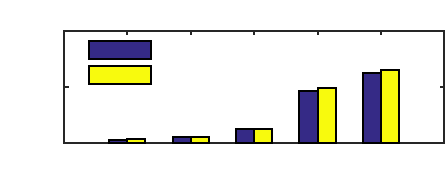
\includegraphics[width=\unitlength]{numberofframessvg.pdf}}%
    \put(0.49756185,0.01128552){\makebox(0,0)[lb]{\smash{\small{t[s]}}}}%
    \put(0.09282368,0.08132461){\makebox(0,0)[lb]{\smash{0}}}%
    \put(0.06443245,0.20731075){\makebox(0,0)[lb]{\smash{50}}}%
    \put(0.03604122,0.33329678){\makebox(0,0)[lb]{\smash{100}}}%
    \put(0.35378421,0.29015447){\makebox(0,0)[lb]{\smash{kinect}}}%
    \put(0.35378421,0.23448302){\makebox(0,0)[lb]{\smash{ensenso}}}%
    \put(0.27065576,0.05747682){\makebox(0,0)[lb]{\smash{1}}}%
    \put(0.41567291,0.05916184){\makebox(0,0)[lb]{\smash{6}}}%
    \put(0.55919591,0.06036764){\makebox(0,0)[lb]{\smash{9}}}%
    \put(0.69462102,0.05909079){\makebox(0,0)[lb]{\smash{25}}}%
    \put(0.83415963,0.05814475){\makebox(0,0)[lb]{\smash{30}}}%
    \put(0.02193696,0.08258763){\rotatebox{90}{\makebox(0,0)[lb]{\smash{\small{Number of frames}}}}}%
  \end{picture}%
\endgroup%
